
\documentclass{mcmthesis}
\mcmsetup{CTeX = false, 
        tcn = 2123705, problem = B,   % 修改控制号和选题号
        sheet = true, titleinsheet = true, keywordsinsheet = true,
        titlepage = false, abstract = true}
\usepackage{palatino}
\usepackage{lipsum}
\usepackage{amsmath}  % 此处引入数学公式的包
\usepackage{graphicx} % 用于插入图片
%%% 实现参考文献标号在右上角
\newcommand{\upcite}[1]{\textsuperscript{\textsuperscript{\cite{#1}}}}
% 控制页 %%%%%%%%%%%%%%%%%%%%%%%%%%%%%%%%%%%%%%%%%%%%%%%%%%%%%%%%%%%%%%%
% 论文标题
\title{The Template for MCM}  % 修改标题
\date{\today}
 
\begin{document}
\begin{abstract}

  First, we determine the location of EOC through a multi-objective planning model. We plan the EOC site selection separately in different terrain. The main considerations are the distance between EOC and each fire point in the jurisdiction, the number of fire points covered by the EOC, the fire frequency of the fire point, and the number of EOCs. We have selected a combination of 5 EOCs to optimize the total benefit.
    
  Second, we use genetic algorithms to plan the flight route of the SSA drone, and according to the rules of forest fires, The SSA drone should check the location of firefighters and the fire situation twice a day. According to the schedule and the shortest inspection route, we calculated that the required number of SSA drones is 13. At the same time, according to the preading speed and the frequency of fire, we established a non-linear programming model and determined that 18 repeater drones are needed to maintain uninterrupted radio communications in the fire spreading area.
      
  After introducing the influence of terrain factors on radio signal transmission into the model, we further optimized the model and introduced some calculation formulas for shadow fading caused by obstacles and the increase of distance during radio transmission. And we calculated the function of radio loss in mountain area with respect to propagation distance,which is applied to our model. After that, we have added a new repeater drone as the modification to the previous model.
      
  Third, to predict the fire events in Victoria over the next decade, we used the BP neural network algorithm and cellular automata. First, according to the climate data and fire frequency of Victoria from 2011 to 2020, we constructed the model by BP neural network algorithm and predict the fire frequency over the next decade. Second, through the simulation of cellular automata, we simulate the direction and trend of fire spreading. So we modified the EOC location model and drones planning model according to the predicted fire event data, so as to determine the changed number of EOC and drones.    
  
  Finally, based on the number and mix of drones, and considering the fire event over the next decade, we gave a budget request to the Victorian government.
      
  Our model for EOC location selection and drones arrangement can cover more than 80\% of the fire-prone areas along the coastline of Victoria, and can ensure that firefighters in the hardest hit areas can communicate with EOC all day. At the same time, The SSA drone's shift schedule ensures that it can traverse every historical fire "flammable point" twice a day.

\begin{keywords}  
Multi-Objective Planning ; BP Neural Network Algorithm;Cellular Automata;
\end{keywords}
\end{abstract}
 
% 目录页 %%%%%%%%%%%%%%%%%%%%%%%%%%%%%%%%%%%%%%%%%%%%%%%%%%%%%%%%%%%%%%%%
\maketitle         % 控制序列
\tableofcontents   % 生成目录
\newpage
 
% 基础用法 %%%%%%%%%%%%%%%%%%%%%%%%%%%%%%%%%%%%%%%%%%%%%%%%%%%%%%%%%%%%%%%
 
% 标题 -----------------------------------------
\section{Introduction}
\subsection{Background}
Australia is the country with the largest area in Oceania and the country with the most serious wildfire problem. On average, more than 50,000 wildfires occur each year and about 50 million hectares of forest grassland are burned. \upcite{c_building}During the 2019-2020 fire season , devastating wildfires have occurred in every state in Australia, with New South Wales and eastern Victoria having the worst impact. Severe drought and continued heat waves are the cause of this wildfire, and climate change has exacerbated this phenomenon. The fire not only caused casualties and extensive land destruction, but also caused the death or displacement of nearly 3 billion animals.

\subsection{Our Work}
\begin{itemize}
\item Determine the location of EOC: We proposed a multi-objective planning model based on the evaluation of fire frequency and distance.

\item Determine the flight path: We used genetic algorithm to calculate the shortest traverse path.

\item Determine the number and mix of drones:  Based on the ratio of the shortest traversal path length of each EOC jurisdiction to the longest distance of the drone flying and the drone scheduling plan we developed.

\item Determine the location of repeater: We established a nonlinear programming model to determine the location of the repeater (based on the evaluation of the fire range).

\item Predict fire events over the next decade: We used time series methods to predict climate conditions and used BP neural network to predict the frequency of fires in each month. We predicted the spreading trend of each extreme fire by cellular automata and analyzed the increase of equipment cost.

\item Propose the budget: We proposed an annotated budget request for Victorian government.
\end{itemize}









\section{Assumptions and Justifications}
\begin{itemize}
  \item All road nodes are positioned at the grid intersection point closest to their actual position, and the error is within an acceptable range.

  \item EOC needs to be established at the intersection of multiple roads in order to transport supplementary materials on the ground in time.
  
  \item The area surrounded by a gray straight line is regarded as a fire occurrence area, and each pixel is regarded as a flammable point. The pixels that cross the area are counted as out-of-area points according to their area ratio in the area. The flammable point is equal to 50\%.
  
  \item The drone can still complete remote sensing positioning and fire monitoring tasks while flying at the highest speed.
  
  \item Drones in plains and mountainous areas will fly at a fixed altitude after taking off because the monitoring location is close to the take-off location, and there will be no altitude changes during the flight.
  
  \item Since the drone’s flight path planning route revolves around the circle centered on the EOC, it can be considered that the number of drones obtained by dividing the total shortest path length by the longest path of a single drone flying upwards is reasonable. It can meet the requirements of the distance required for recharging the drone midway.
  
  \item All drones finally return to the starting point after departure from EOC, there is no drone's round-trip between EOC.
  
  \item The impact of the flying height of the drone on the communication coverage with a radius of 20km is negligible.
  
\end{itemize}



\section{Notations}
Here are the notations and their meanings in our paper:

\begin{center}
  \begin{longtable}{p{.1\textwidth}p{.8\textwidth}m{.4\textwidth}}
  \caption{The List of Notation}\\
  \hline
  Symbol& Meaning \\
  \hline
  
  $F_{i,j}$      & the point where the fire has occured before, with the coordinate of (i,j)\\
  $O_{m,n}$      & the EOC point, with the coordinate of (m,n)\\
  $RP_{p,q}$    &   the Radio Repeater drones, with the hovering coordinate of (p,q)\\
  $y_{i,j,m,n}$   &  a 0-1 variable shows whether the  $F_{i,j}$ is in the durisdiction of $O_{m,n}$ \\
  $Dis_{i,j,m,n}$     &  the distance between  $F_{i,j}$ and $O_{m,n}$  \\
     $R_{DP}$  &  the max radius of the drone's flight\\
     $R_{RP}$ &  the max radius of the Radio Repeater's communication \\
     $R_{RA}$ &  the max radius of the handheld radio's communication
     \\
     $F_{i,j}$ &  the rank of fire frequency in  $F_{i,j}$
     \\
     $k_{i,j}$&  the rank of the drone's speed when flying across  $F_{i,j}$
     \\
     $D_{max}$ &  the max distance a drone can cover\\
      $T_{max}$ &the max time a drone can fly   \\
       $V_{max}$&   the max speed a drone can reach       \\
     $T_{charge}$  & the time for charging of a drone  \\
     $Num_{EOC}$ & the number of EOC  \\
     $Num_{RP}$ &  the number of Radio Repeater drone     \\
     $Num_{F}$         &    the number of the points where the fire has occured before     \\
     $NumF_{P}$        &  the number of the points which meet the demand of P\\
     $L_{m,n}$& the shortest path of traverse points in EOC  \\
     $NumD$ &the number of SSA drones\\
    $\overline{V} $ & the average flying speed of the drone\\
     $t$ & patrol time for a flight\\
  \hline                                                       
   \end{longtable}
   \end{center}



\section{Multi-Objective Programming Model for the Choice of EOC Location}
\subsection{Data Acquisition and Preprocessing}
We obtain historical fire data of Australia from FIRMS\upcite{fire_website} which include latitude and longitude information, fire's occurrence time, fire intensity, etc.

After the filtering of latitude and longitude and other processing, the fire data of Victoria from 2019 to January 2020 are obtained, and the frequency of fire occurrence in each location in the area we reasearched is visualized as a fire frequency distribution map.It is consistent with the image results on the website.

Through the conversion of longitude and latitude with the actual distance, the fire area of Victoria was projected to a two-dimensional coordinate plane system. Suppose that the longitude and latitude coordinates of the inflection points in the peripheral area of the map are$ (x_1, y_1)$ and$ (x_2, y_2)$ , the conversion formula between the longitude and latitude of the original map and the two-dimensional plane coordinates is as follows (R is the radius of the earth, usually equal to 6370km):

$Dis=R*arccos(siny_1*siny_2+cosy_1*cosy_2*cos (x_1-x_2))$

The two-dimensional plane projection drawing after coordinate conversion is as follows, in which the scaling ratio between the coordinate value and the actual distance (km) is 1:1.25.

        \begin{figure}[H]
            \centering
            % \subfigure[图1]
            {
            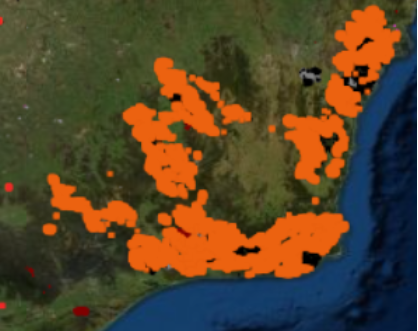
\includegraphics[width=0.45\textwidth]{image/firemap.png} 
            }
            % \subfigure[图2]
            {
            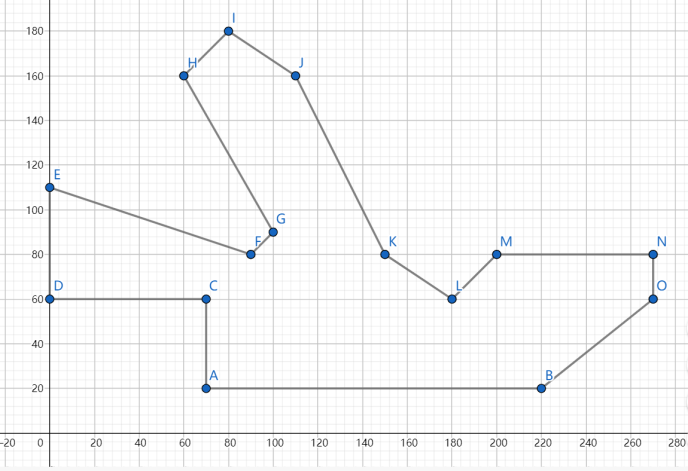
\includegraphics[width=0.45\textwidth]{image/1.png}
            }
            \caption{Fire image map and converted coordinate map\upcite{fire_website},
            The boundary in the left image is approximately the boundary between Victoria and New South Wales}
            \label{png1}
        \end{figure}

\subsection{How Do We Choose EOC Location}
After a disaster, EOC is dispatched and placed in the vicinity of the disaster site. EOC is usually a large vehicle loaded with material resources that may be needed in the process of the disaster relief, such as medical and health equipment, maps of the area, environmental monitoring equipment, and experts are also needed. After coming to the disaster site, EOC will be deployed near the site of an emergency, and will not move again until the rescue was finished. 

Since it is almost impossible for heavy vehicles to go deep into the fire center through the burning forest, we suggest that EOC must be built near the roads. And in order to make the material transportation more convenient, we suggest that EOC should be deployed at the intersection of the main roads. The figure below marks the main road distribution of the fire spreading area of Victoria. We also mapped it to the two-dimensional coordinate plane, and approximate the tortuous road to a straight line with inflection points. We have marked all the main turning points of roads in the fire area:

\begin{figure}[H]
  \centering
  % \subfigure[图1]
  {
  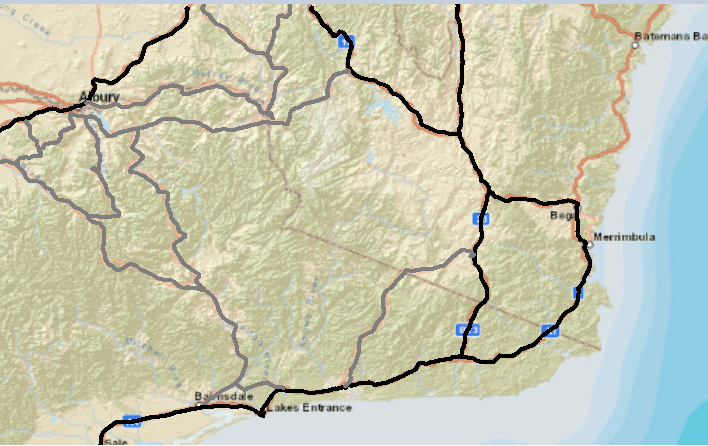
\includegraphics[width=0.45\textwidth]{image/2.png} 
  }
  % \subfigure[图2]
  {
  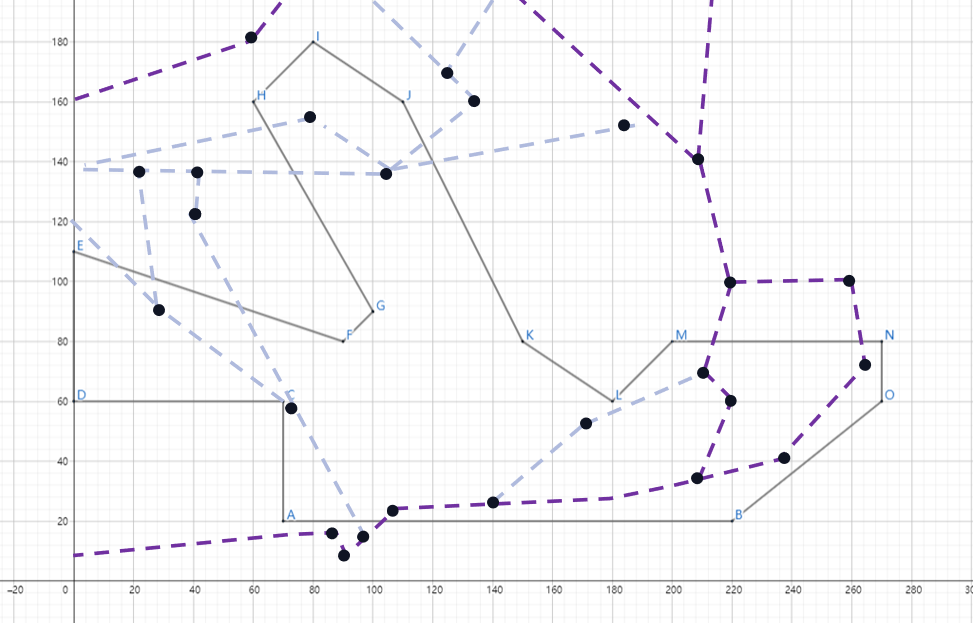
\includegraphics[width=0.45\textwidth]{image/3.png}
  }
  \caption{Road distribution map and converted coordinate map\upcite{fire_website}
  % The boundary in the left image is approximately the boundary between Victoria and New South Wales
  }
  \label{png1}
\end{figure}


The purpose of EOC location optimization is to maximize the work efficiency of drones. Since the Bogong mountain with an altitude of 1986m stretches from the northeast to the west of Victoria, and there is a plain area with an altitude of less than 300m on the edge of the coastline, we set up EOC in the high mountain area and the plain area respectively to cover the surrounding area which has almost the same height with the take-off point considering the travel loss of drones caused by flying over the mountains. The impact of mountain area on EOC must be considered when setting up EOC at the abrupt elevation.Therefore, we need to obtain the terrain distribution and altitude data of Victoria.

First of all, we obtained the hierarchical color map of Victoria (which uses color saturation and brightness transformation to identify the characteristics of landform morphology and height distribution\upcite{c_height}).

According to the mapping relationship between color and altitude in the map, the altitude value of each point in this area is obtained, and a three-dimensional altitude map of this area is drawn by interpolation fitting method.

\begin{figure}[H]
  \centering
  % \subfigure[图1]
  {
  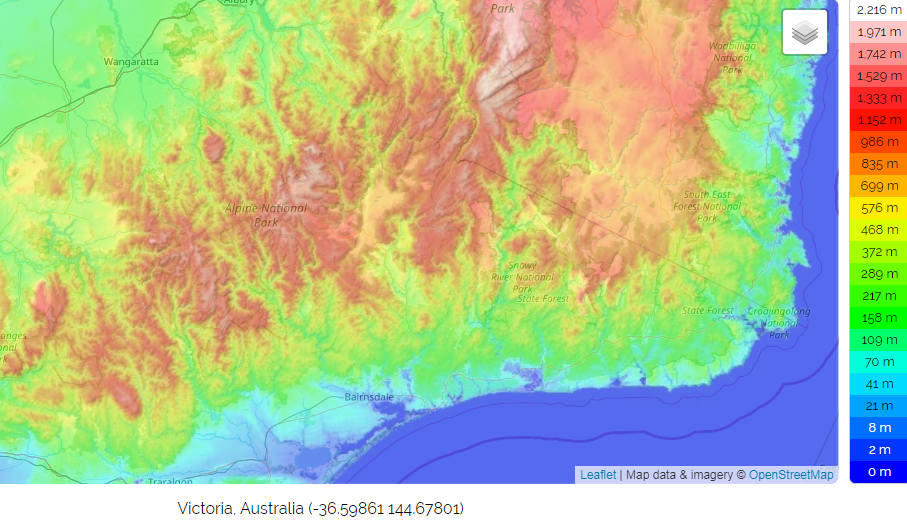
\includegraphics[width=0.45\textwidth]{image/colormap.png} 
  }
  % \subfigure[图2]
  {
  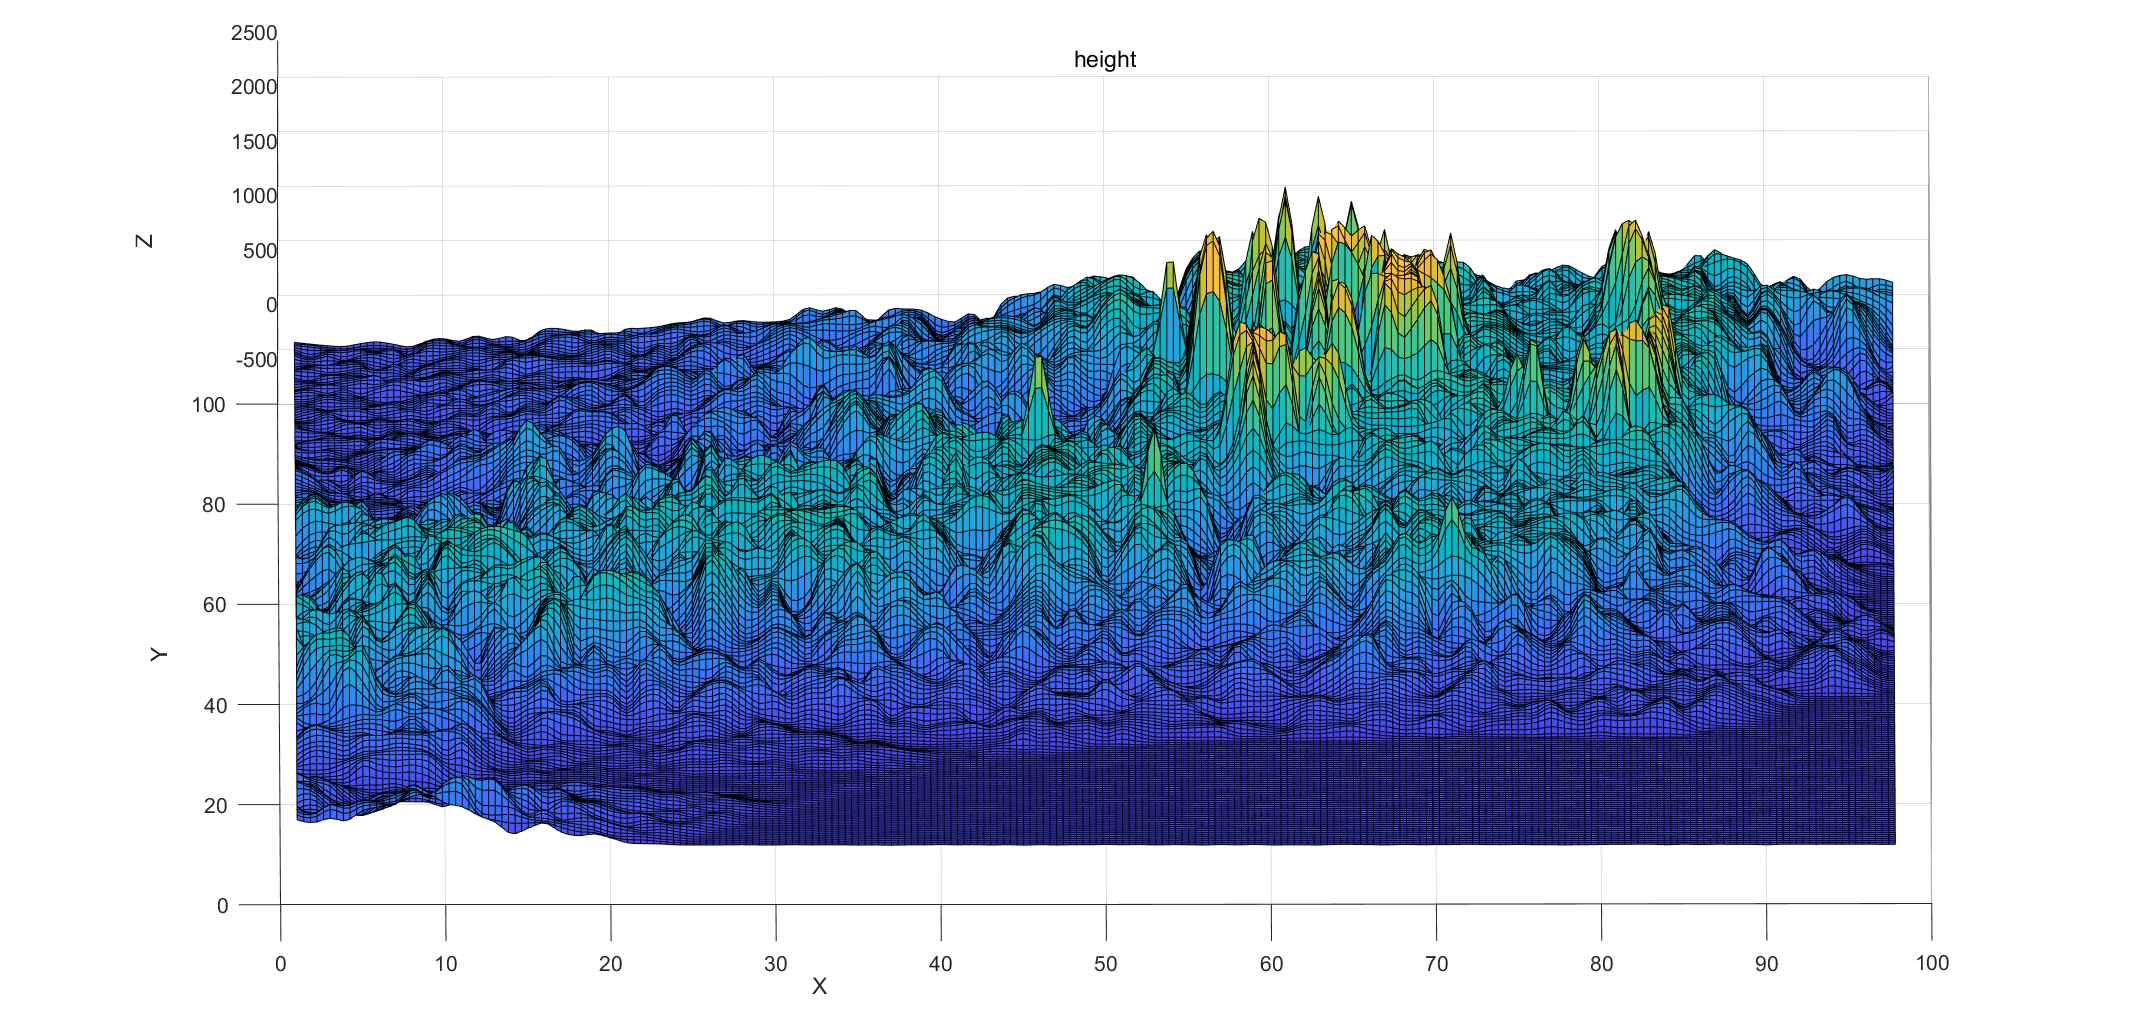
\includegraphics[width=0.45\textwidth]{image/Height.png}
  }
  \caption{the hierarchical color map and altitude map of Victoria}
  \label{png1}
\end{figure}


The fire area is divided into three parts according to the altitude map: plain area, mountainous region and transitional zone.

\begin{figure}[H]
  \centering
  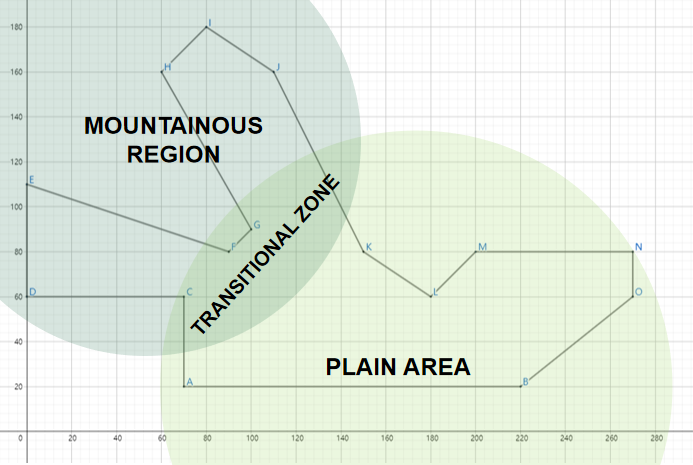
\includegraphics[scale=0.4]{image/4.png}
  
  % \label{png1}
\end{figure}

The main task of SSA drones is to obtain the location of fire fighters through wearable devices, and monitor the fire spreading trend through high-definition and thermal imaging cameras and telemetry sensors. For safety reasons, EOC should be set where the drones can reach as many conflagration areas as possible, obtain as many data of the fire fighters as possible, monitor the spreading of the fire as fast as possible, ensure the safety of fire fighters and report the fire spread trend in time. For financial reasons, the layout of an EOC requires a lot of human and material resources. So the number of EOC should be as small as possible on the premise of meeting most of the needs. Therefore, we established a multi-objective programming model to find the best amount and location of EOC .


\subsection{Model Construction}


Planning Objective 1: maximizing the number of flammable points within the range of drones flight starting from EOC.

\begin{center}
  $max\ NumX\{\left \| \overrightarrow{F_{i,j}O_{m,n} }  \right \| \le R_{DR}\}$
\end{center}



Considering that on the premise of meeting the mission requirements, the flight distance of drones should be shortened as much as possible, and the frequency of fire should also be taken into account. The formula above can be transformed into:

\begin{center}
  
$
max~z=\sum_{i}^{} \sum_{j}^{} \sum_{m}^{} \sum_{n}^{} y_{i,j,m,n}\frac{f_{i,j}}{Dis_{i,j,m,n}} 
=\sum_{i}^{} \sum_{j}^{} \sum_{m}^{} \sum_{n}^{} y_{i,j,m,n}\frac{f_{i,j}}{\left \| \overrightarrow{F_{i,j}O_{m,n}}  \right \| } 
=\sum_{i}^{} \sum_{j}^{} \sum_{m}^{} \sum_{n}^{} y_{i,j,m,n}\frac{f_{i,j}}{ \sqrt{(i-m)^2+(j-n)^2}   } 
$


$
y_{i,j,m,n}=
\begin{cases}
  & \text{ 0 }~~when~ F_{i,j}~ is ~out ~of ~ the ~monitor ~range ~of ~the ~SSA ~from ~O_{m,n}  \\
  & \text{ 1 }~~ when~ F_{i,j}~ is~ in ~ the~ monitor~ range ~of ~the ~SSA ~from ~O_{m,n}  \\  
\end{cases}
$

$
f_{i,j}=\begin{cases}
  & \text{ 0 }~~ when~ the ~frequency~ of ~fire~ is~ in~ F_{i,j} ~\in ~[0,5] \\
  & \text{ 1}~~ when~ the ~frequency~ of ~fire~ is~ in~ F_{i,j} ~\in ~[6,100] \\
  & \text{ 1.5}~~ when~ the ~frequency~ of ~fire~ is~ in~ F_{i,j} ~\in ~[101,300] \\
  & \text{ 1.8}~~ when~ the ~frequency~ of ~fire~ is~ in~ F_{i,j} ~\in ~[301,+\infty ] 
\end{cases}
$
\end{center}

Planning Objective 2: minimizing the number of EOC

\begin{center}
  $min\ Num_{EOC}$
\end{center}


Constraints: the drones should be located on the road intersections in the plain area or mountainous area.

\subsection{Model Solving}

Based on the fire frequency data of this area, we calculated the sum of fire frequency of each area block with 5km interval in the conflagration area, and draw the frequency chart with MATLAB according to the fire frequency as follows, in which the brighter area represents the higher fire occurrence frequency.

\begin{figure}[H]
  \centering
  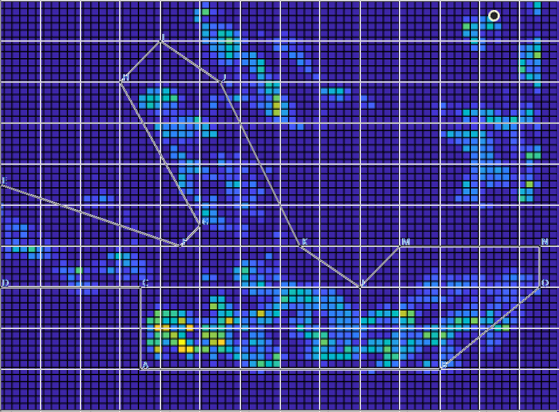
\includegraphics[scale=0.4]{image/5.png}
  % \caption{ss5555}
  % \label{png1}
\end{figure}

At the same time, we calculate the distance from each grid covered by the circle with a radius of 30km and a road intersection as the center (EOC), and evaluate each road intersection by computer programming.

The evaluation standard is proportional to "the frequency of fire multiplied by the reciprocal of the distance to EOC", the higher the frequency, the closer the EOC location, the larger the result, the more reasonable the EOC address is.

Its significance is that the EOC should be as close as possible to the area with serious fire, so that the drones can take off from EOC more conveniently.

We need to determine the number of EOC, and the final result should make the total covered effect of all selected EOC win the highest score. So we traversed 23 road intersections except the one in the transition zone between mountainous and plain area. The coverage effects and economic benefits rise to an ideal level when we choose to establish five EOC, and the addition of the fifth EOC greatly increased the score of the original four EOC. The road intersection is selected as follows:

\begin{figure}[H]
  \centering
  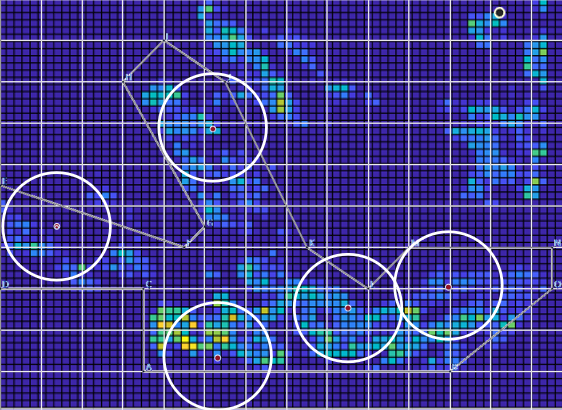
\includegraphics[scale=0.4]{image/6.png}
  % \caption{ss}
  % \label{png1}
\end{figure}


\subsection{Model Optimization Based on Terrain and Communication Range}

We considered the transition zone between the plain and mountainous area, and the impact of the additional 20km radio range of Radio Repeater drones on the existing evaluation results. Firstly, change of flight distance caused by mountainous terrain should be considered (assuming that the cross profile of the mountain is a triangle).

\begin{figure}[H]
  \centering
  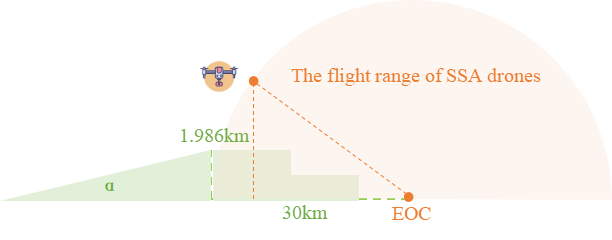
\includegraphics[scale=0.4]{image/7.png}
  % 
  % \label{png1}
\end{figure}

Since the side of Bogong Mountain located near the conflagration area is mainly cliff, it is not scientific to calculate the increase of drones' flight distance through the hypotenuse of the triangle. We assume that when the drone encounters an obstacle, it will fly parallel to the ground after flying over the altitude, and continue to increase the flight altitude vertically until it encounters the next obstacle. Therefore, the flight distance of the drones in the transition zone between mountain and plain is about 2km, which expands the flight range of drones and affects the remote control of drones by EOC. After calculation, the height of the mountain reduces the radius of its flight range by about 0.1km. Since this value is quite small relative to 30km, we still calculate the flight range of drones in the transition area by 30km.

After considering the signal range of repeater which is 20km, we used the signal receiving range of EOC under the effect of repeater to measure the scope of jurisdiction. According to the sum of the communication diameter of repeater and the communication radius of handheld radio equipment, we determine that the radio communication coverage of EOC is 20 + 20 + 5 = 45km. We traversed 24 road intersections of the whole map again, and calculate the distance with the optimal combination of five EOCs. It is found that the best five coordinates have changed. The smaller circle in the figure represents the flight range of SSA drones, and the larger circle represents the potential signal receiving range of Radio Repeater drones.

\begin{figure}[H]
  \centering
  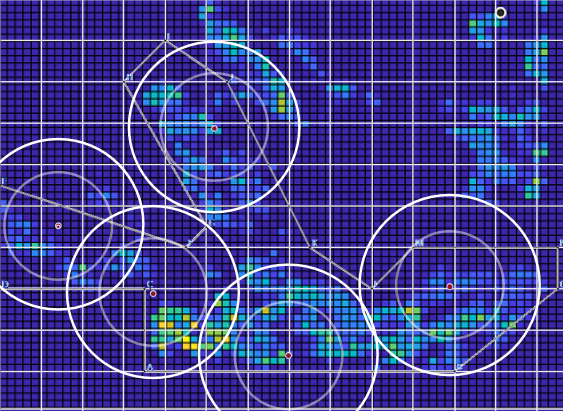
\includegraphics[scale=0.4]{image/8.png}
  
  % \label{png1}
\end{figure}

The scores of all the points are as follows. We draw a six dimensionals scatter diagram through python. D1-D5 are the id (1-23) of the five EOC positions, and the size of the point represents the value of the function.

\begin{figure}[H]
  \centering
  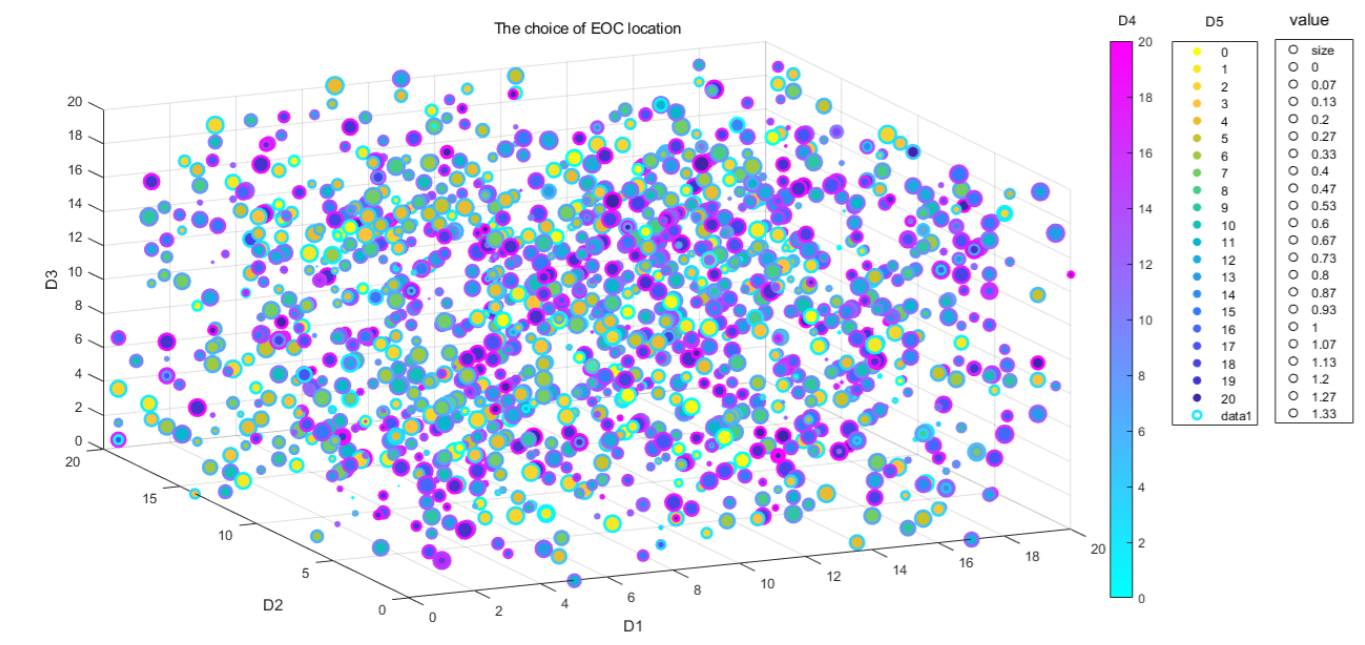
\includegraphics[scale=0.4]{image/9.png}
  
  % \label{png1}
\end{figure}


The corresponding coordinates of the new optimal intersection number are  (6,25), (20,16), (38,8), (28,39), (58,17). So far, we have determined the optimal number and location coordinates of EOC.


\section{Optimizing of the Number of Drones Based on Genetic Algorithm}


\subsection{Determination of the Number of SSA Drones}
\subsubsection*{5.1.1 Establishment of Genetic Algorithm Model}
Genetic algorithms (GA) is an optimization method that simulates the natural selection in the biological world. Its essence is to get the optimal solution or quasi optimal solution through group search technology and evolution generation by generation according to the principle of survival of the fittest.

According to the process of natural selection, the steps of genetic algorithm are determined.

\begin{itemize}
  \item Generation of the initial population: determine the coding method and initial population.
  In this paper, decimal coding is adopted, and random sequence $w_1-w_{Num_F+2}$ acts as chromosome. Each random sequence corresponds to an individual in the population.
  The coded position i represents the target i, and the random number of position i represents the sequence of target i in SSA investigation.

  \item First,we use the classical approximation algorithm:improved ring algorithm to get a better initial population.
  \item Calculate the fitness rank of each individual: determine the fitness function (minimum total length of drones' flight path) and evolution parameters (set to 50).

  \item According to the principle of survival of the fittest, excellent individuals are selected; And according to the fitness function, some solutions with larger total length of flight path would be eliminated.
  \item The next generation population was generated by randomly crossing chromosome genes and random variation: Determine the probability of crossover and mutation.
  \item According to the mutation rate given at first, three integers are randomly selected from the selected individuals to meet the requirements of $1 < u  < v < w < 26$.
  Insert the gene segment between u and v (including u and V) to the position after w.
  \item Select M (sets 5) individuals with the minimum objective function value to evolve to the next generation.

\end{itemize}



\subsubsection*{5.1.2 Model Solving}

We use genetic algorithm to solve. Taking EOC as the center and the maximum flight range of the UAV (30km) as the radius delineated area, the shortest flight path of the SSA UAV corresponding to the five EOCs is finally obtained as follows:

\begin{figure}[H]
  \centering
  {
  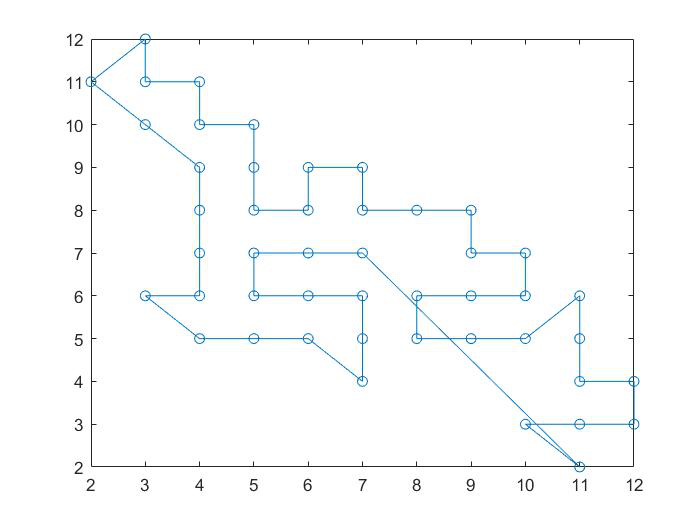
\includegraphics[width=0.3\textwidth]{image/A.png} 
  }
  {
  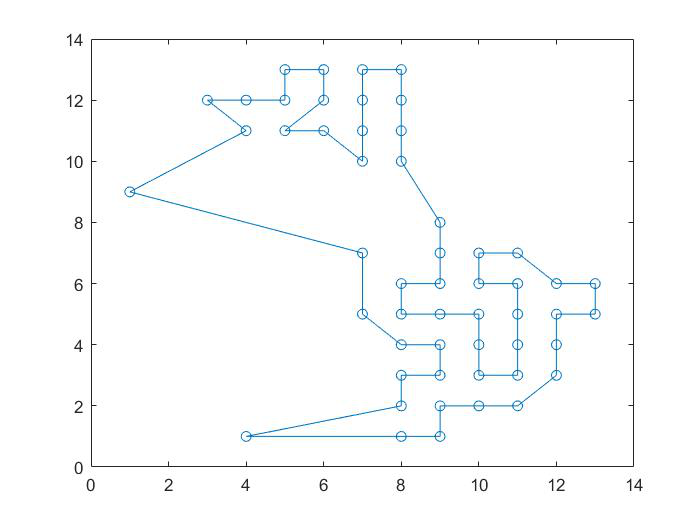
\includegraphics[width=0.3\textwidth]{image/B.png} 
  }
  {
  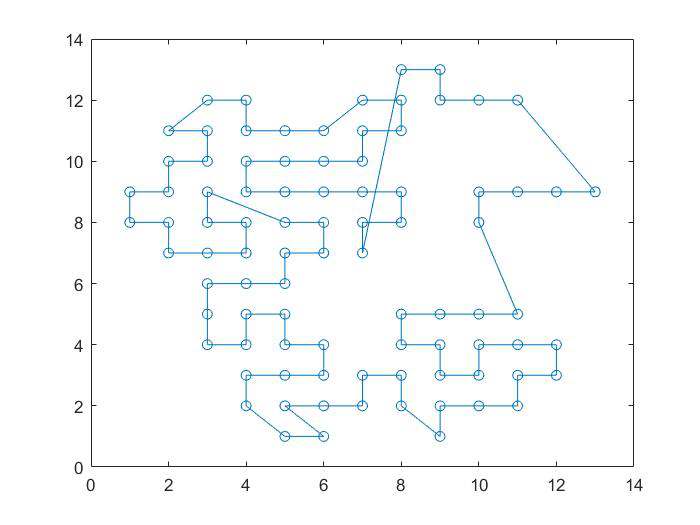
\includegraphics[width=0.3\textwidth]{image/C.png}
  }
  % 
  % \label{png1}
\end{figure}

\begin{figure}[H]
  \centering
  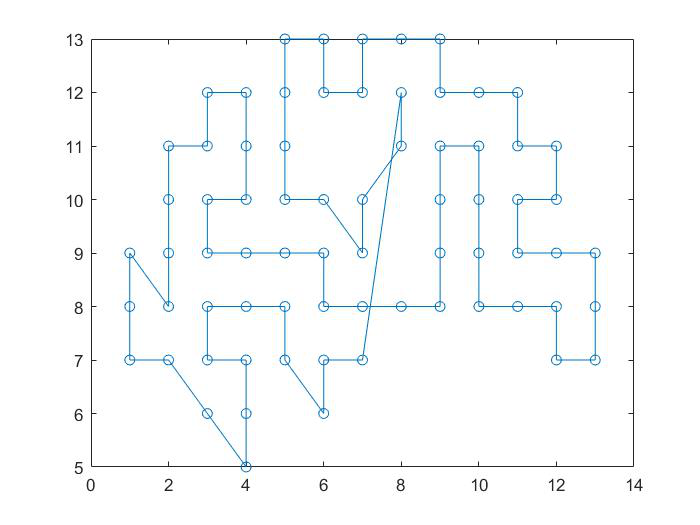
\includegraphics[width=0.3\textwidth]{image/D.png} 
  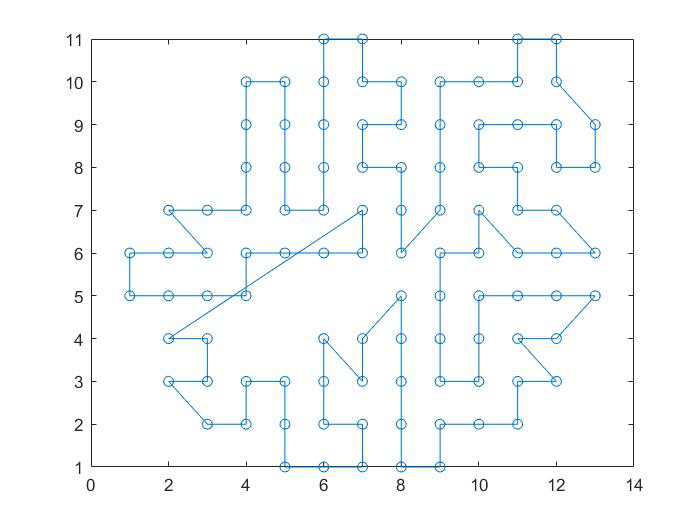
\includegraphics[width=0.3\textwidth]{image/E.png} 
  \caption{the shortest flight path}
  % \label{png1}
\end{figure}

Taking one of the EOC as an example, the longest flight distance of drones is:

$D_{max}=T_{max}*V_{max}$

Taking t hour as the length of shift, assuming that the drone taking off from EOC in Ti , the number of drones required to traverse all flammable points in a shift is as follows:

$Num_D=\left \lceil \frac{L}{t\overline V}  \right \rceil $

Among them,
$\overline{V}=\frac{ \sum_{i=1}^{n}  k_{i,j}V_{max} }{Num_{F}}  $


According to the research made by ZhengLinyu\upcite{4_best}, the high incidence period of forest fires is from 10am to 4pm, accounting for 80% of all forest fires, among which the fire incidence from 10am to 2pm accounts for 46.7%. Therefore, the best fire inspection frequency is as follows:

\begin{center}
  \begin{tabular}{|r|r|r|}
    % r代表row, 使用 | 来划分,如果 r | r中间的|去掉,那么列之间元素无直线划分
    \hline
    No.&Starting time of the flight &The lasting time of each flight \\ \hline
    1&10:30&  2.5h \\ \hline
    2&15:00 & 2.5h \\ \hline
    \end{tabular}
\end{center}

According to the calculation results, the SSA drone needs to pass 244.4975km to traverse the fire point within the first EOC range. According to the drone's flying speed of 20m/s and the flight time of 2.5 hours, at least 2 drones are required to cover this distance. It takes 327.25km to traverse the fire point within the second EOC range, at least 2 drones are required to cover this distance, and 475.4km to traverse the fire point within the third EOC range, and this distance needs to be at least 3 drones, traversing the fire point within the fourth EOC range requires 362.43km, covering this distance requires at least 3 drones, and traversing the fire point within the fifth EOC range requires 520.71km,  3 drones are required for this journey. Therefore, we need a total of 13 SSA drones.


\subsection{The Determination of the Number of Radio Repeater Drones}


\subsubsection*{5.2.1 Model Construction}

Because SSA drones can effectively cover flammable points within a 30km radius of the EOC, radio repeaters will hover at the edge of the circle after reaching the 30km circle from the EOC in order to maximize the regulated area. The determination of the radio repeater drones is mainly accomplished by traversal of each point in the circle area with EOC as the center and 20km as the radius. We calculate the amount of the points within the range of 25km around the coordinate, and use 0-1 variables calibration to identify if the point had witnessed more than 5 fires. After modifying the EOC location model, we apply to the radio repeater drones location selection as follows:

Planning Goal 1: Maximize the number of flammable points within the radio repeater drone communication coverage:
\begin{equation}
  max\ Num_F\{\left \| \overrightarrow{F_{i,j}RP_{p,q} }  \right \| \le R_{RP}+R_{RA}\}
\end{equation}


Planning goal 2: minimize the number of repeater drones:
\begin{equation}
min\ Num_{RP}
\end{equation}

Constraint conditions: the radio repeater drone shall be located on the circumference of EOC as the center and 20km as the radius, that is:
\begin{equation}
\left \| \overrightarrow{O_{m,n}RP_{p,q} }  \right\| \le R_{RP}
\end{equation}


The final determined number and position of the repeater drones are shown in the figure. We need 9 repeater drones at one time. Considering the charging time of the drones, 18 repeater drones can make sure the EOC keeps in touch with the rescue team during the whole process:

\begin{figure}[H]
  \centering
  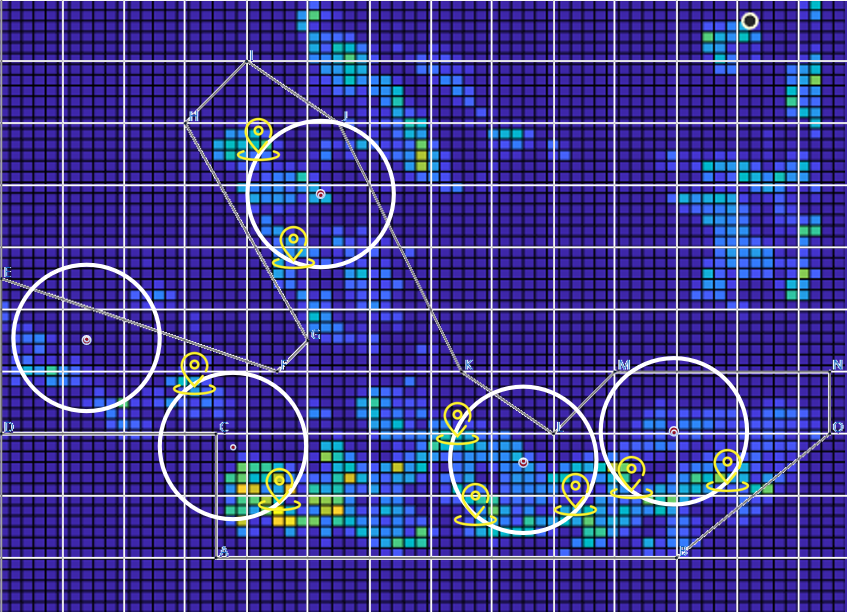
\includegraphics[scale=0.4]{image/F.png}
  
  % \label{png1}
\end{figure}


\subsubsection*{5.2.2 Model Optimization Based on Shadow Fading Factor}

After searching the relevant materials, we found that the undulation of terrain has a great impact on the communication of wireless equipment. The communication distance of handheld wireless equipment may be shortened by more than 60% due to the influence of different terrain, and the repeater will also be subjected to certain interference. Therefore, we must consider the terrain factors and the distance between Radio Repeater drone and handheld radio communication equipment.

The research of Frii\upcite{c_trans} shows that in free space, with the influence of the distance between the radio transceiver and the receiver, the received radio power $P_r (d)$ of the receiver can be represented as: 

\begin{equation}
P_r(d)=\frac{P_1G_1G_r\lambda ^2}{(4\pi ^2)d^2L}
\end{equation}

Where d is the distance between the transmitter and the receiver, $G_t$ is the transmission gain of the transmitting antenna when an anisotropic antenna is used, and $G_r$ is the transmission gain of the receiving antenna. $P_t$ is the transmission power of the radio signal, $\lambda$  is the transmission wavelength, L is the system loss coefficient independent of the environmental variables, indicating the loss of transmission media, filtering and antenna equipment used in the communication process between the transmitter and the receiver. In the ideal state, let $L = 1$, which means that the equipment loss is not considered. In this case, the formula can be converted to :

\begin{equation}
PL_F(d)[dB]=10log(\frac{P_t}{P_r} )=-10log(\frac{G_1G_r\lambda ^2}{(4\pi)^2d^2} )
PL_F(d)[dB]=10log(\frac{P_t}{P_r} )=20log(\frac{4\pi d}{\lambda})
\end{equation}

When the influence of terrain on radio signal transmission is taken into account, we add the path loss index n which changes with the environment to modify the free space path loss model. The logarithmic distance path loss model can be expressed as :
\begin{equation}
PL_{LD}(d)[dB]=PL_F(d_0)+10nlog(\frac{d}{d_0} )
PL_{LD}(d)[dB]=\overline{PL}(d)+X_\sigma=PL_F(d_0)+10nlog(\frac{d}{d_0} )+X_\sigma 
\end{equation}

$d_0$ represents the effective reference range of the model. When n = 2, it corresponds to the infinite electrical signal transmission in the free space. When the number of obstacles increases, n will continue to increase. Generally, in the urban environment, n is defined as 3-4, while in the interior of buildings, n is set as 4-6. When the power of UHF repeater is 3000MHz, we think n = 2 in plain area, and n= 3 in mountainous area and transition area between plain and mountain area. After substituting the above formula, the radio loss rate at each distance is calculated. The curve of loss rate with communication distance is obtained as follows:

\begin{figure}[H]
  \centering
  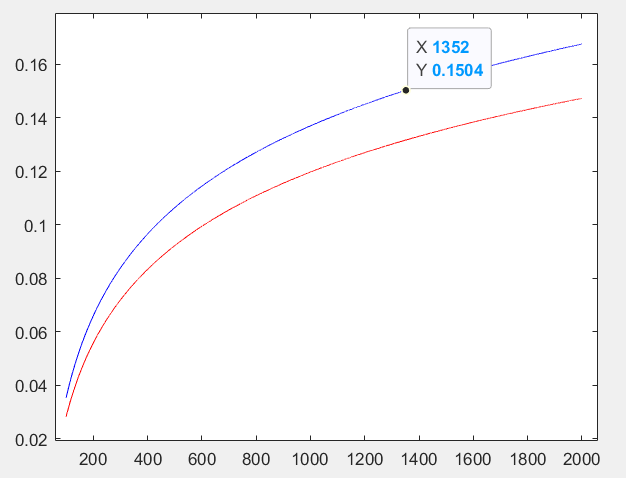
\includegraphics[scale=0.4]{image/G.png}
  
  % \label{png1}
\end{figure}
Generally, we think that signal distortion will occur when the radio loss rate reaches 15\%. It can be seen that in the transition zone of mountainous and plain area, the signal transmission range of repeater carried by drone is reduced to about 13.5km. Therefore, we have narrowed the calculation range of Radio Repeater drone taking off from EOC, and set $R_{RP}$ = 13.5km. Similarly, we have adjusted the propagation distance of handheld radio signal to 2km. After calculation, it is found that a new Radio Repeater drone should be added in, and the new repeater coordinates are as follows:

\begin{figure}[H]
  \centering
  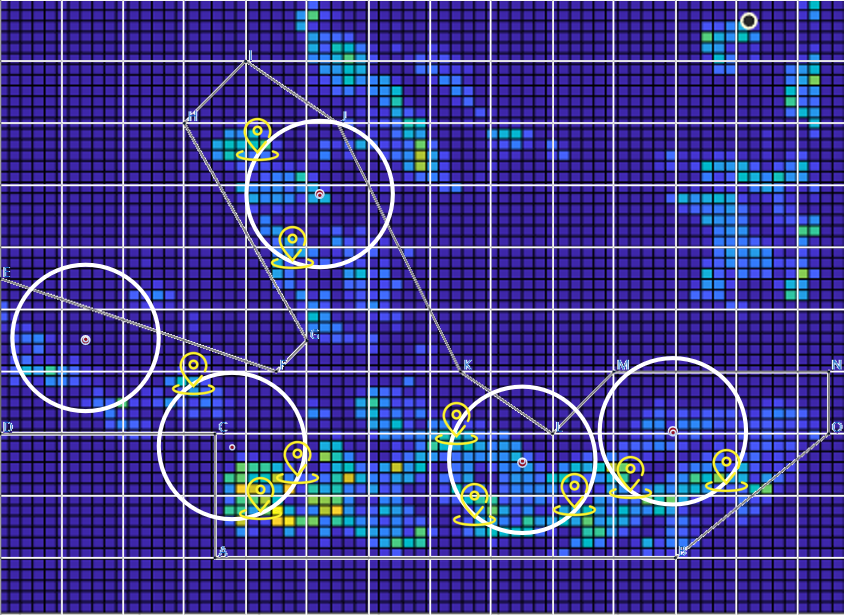
\includegraphics[scale=0.4]{image/H.png}
  
  % \label{png1}
\end{figure}



\section{Forest fire prediction model based on BP artificial neural network}
The occurrence of forest fires is affected by many factors. The terrain factors mainly include altitude, slope, etc.The combustible factors mainly include vegetation type, vegetation coverage, and combustible moisture content; climate aspects mainly include temperature, relative humidity, precipitation and wind speed, etc. Fire source mainly includes fire source type, heat source size, temperature, etc. Therefore, the occurrence of forest fires is a very complex phenomenon.

Because artificial neural networks have strong fault tolerance and highly nonlinear dynamic systems adapt to the random and complex nonlinear occurrence of forest fires, we will use it to simulate and approximate Arbitrary non-linear function and non-linear dynamics of fire occurrence. \upcite{c_BP}The main factors commonly used in the current forest fire forecasting research are temperature, humidity, precipitation, and wind speed. Therefore, on the basis of analyzing the historical data of forest fires in Victoria from 2011 to 2020, we selected the four meteorological factors that affect forest fires, and analyzed the occurrence of fires through the BP artificial neural network model. And use the predicted climate change in Victoria over the next decade to predict the frequency of fires, so that our model can better adapt to fire changes.

\subsection{Data Acquisition and Preprocessing}
\begin{itemize}
  \item Climate data
  
  We obtained monthly climate data from 2011 to 2020 from the Australian government's bureau of meteorology\upcite{climate_website}, and selected Yarrawonga which is the nearest meteorological bureau station  to Victorian island (-35.96. S, 145.95. E) for observation . Our selected climate data indicators are average temperature, average relative humidity, average precipitation, and average wind speed.
  
  \item Fire frequency data
  
  We collected data about fire frequency of Australia from 2011 to 2020 from FIRMS\upcite{fire_webcite}, and obtained monthly fire frequency data of Victoria from 2011 to 2020 by filtering longitude and latitude information.

\end{itemize}

\subsection{Climate Forecast of 2021-2030}

We use a weighted moving average algorithm to predict changes in temperature, humidity, precipitation, and wind speed in the next ten years. The more recent data have a greater impact on the predicted value, so we use the monotonically increasing decimal method to determine the weight, giving a larger weight to the recent data and a smaller weight to the long-term data.

The calculation formula is: $Y_t={\textstyle \sum_{i=1}^{k}}w_{t-i}Y_{t-i}$
and The meaning of each symbol is:
$t$ is time series subscript,
$w_{t-i}$ is the weight of the $t-i$ period (the sum of the weights is 1),
$Y_t$ is actual value of period $t$,
$k$ is number of observations.

So we can predict the changes in temperature, humidity, precipitation, and wind speed in Victoria from 2021 to 2030.

\subsection{Forecast of Fire Events from 2021 to 2030}

According to the climate data from 2011 to 2020, the BP neural network model is built using matlab's newff function.

In theory, when the number of hidden layers is 1, it can fit any function that contains a continuous mapping from one finite space to another finite space.

The number of hidden layer nodes has an impact on the performance of the neural network. According to the empirical formula

$h=\sqrt{m+n}+a$

Among them, h is the number of hidden layer nodes, m is the number of input layer nodes, n is the number of output layer nodes, and a is an adjustment constant between 1-10.

So we first build the network, set the number of different network neurons and the number of network layers within this range.Next,we compare the error accuracy of the experimental results through multiple experiments to find the optimal parameters. Finally we decide to use 2 hidden layers, and the number of nodes in each layer is 50 .

The transfer function of the hidden layer is tan-sigmoid, and the transfer function of the output layer is linear. The training function is traind.

We tried to build the model in units of 5 and 10 years, and finally the latter got better results.

Based on the predicted climate data from 2021 to 2030, this model is used to predict the frequency of fires in each month over the next decade. We get the fire's trend and compare it with the past 10 years as shown in the figure.

\begin{figure}[H]
  \centering
  % \subfigure[图1]
  {
  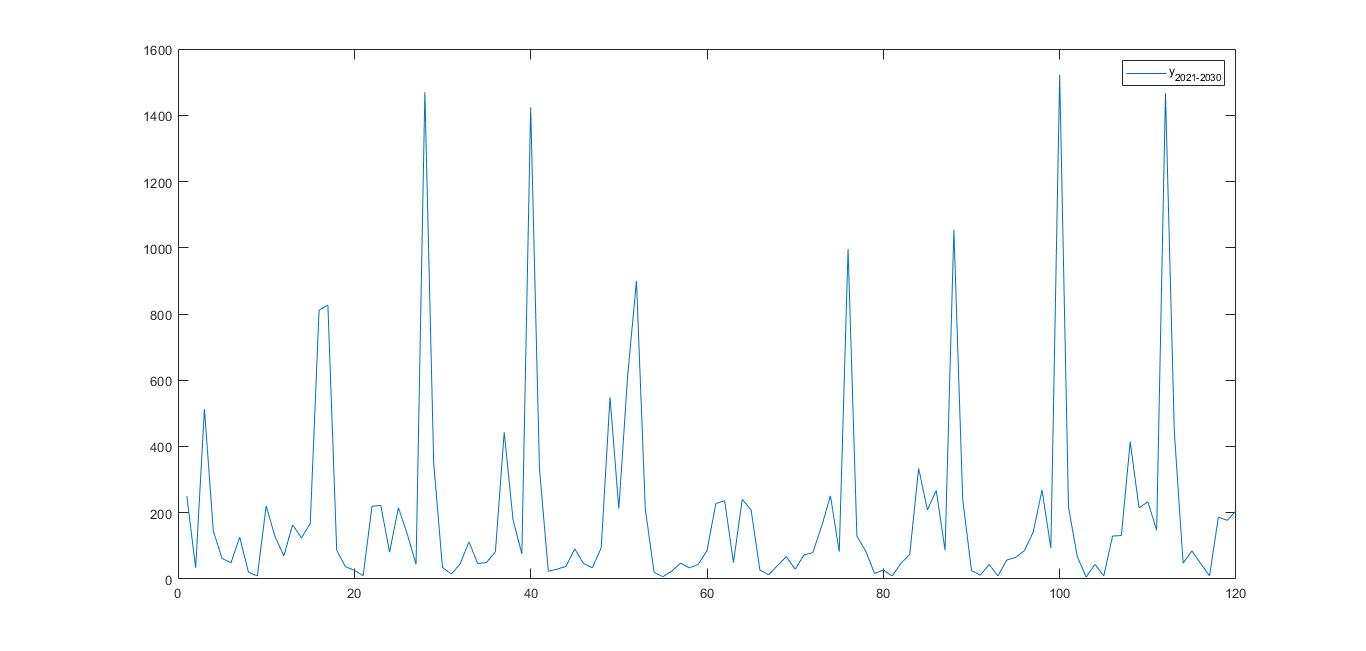
\includegraphics[width=0.4\textwidth]{image/y_21_30.png} 
  }
  % \subfigure[图2]
  {
  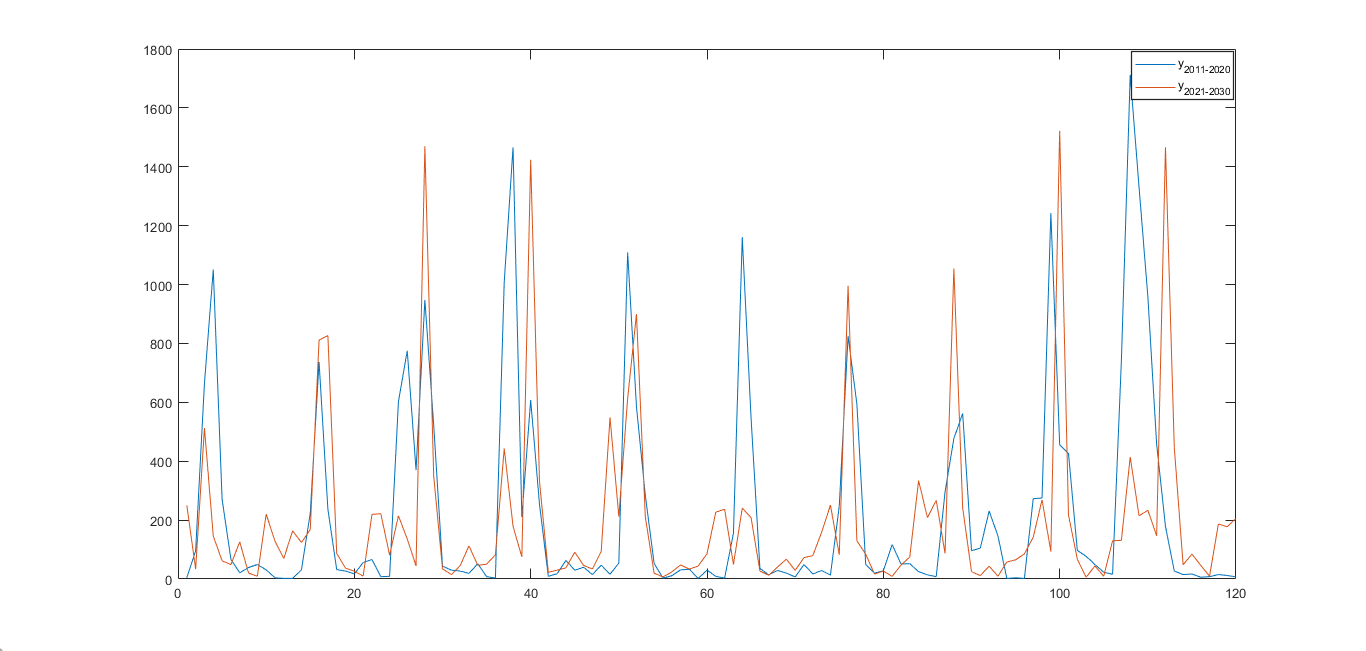
\includegraphics[width=0.4\textwidth]{image/compare_10_10.png}
  }
  \caption{Forecast of Fire Events from 2021 to 2030 }
  \label{png1}
\end{figure}




\section{Prediction Model of Fire Spread Trend Based on Cellular Automata}

\subsection{Model Construction}

Cellular automata CA includes cellular N, neighborhood NC, state S and rule R. A cellular automata system can be represented as :
\begin{center}
$CA=(N,S,NC,R)$
\end{center}

The cell is the smallest unit in the cellular automata, which is used to discrete and divide the complex system in the dimensions of space and time. The unit has constant state at a certain coordinate position in acertain time slice. The state of each small unit in a time slice only depends on the state of its neighborhood unit and its own state in the previous time slice. Cellular automata works the same as the forest fire spreading model, in which each plant acts as a cell, and its state can be represented as :

\begin{equation}
S_{x,y,z}=
\begin{cases}
  & \text{ 0 }\ ~~\   there\ is\ no\ combustible\ here \\
  & \text{ 1 }\ ~~\   the\ combustible\ is\ not\ burning\\
  & \text{ 2 }\ ~~\   the\ combustible\ is\ burning
\end{cases}
\end{equation}

Considering the impact of mountainous topography on the spread rate of forest fires in Victoria, we use the three-dimensional coordinate plane to define the location of cells. We believe that only the burning cells can infect their neighborhood. We take 26 units around the cell as its field, and each infection effect only works within the neighborhood of the burning cell.

The heated air in the equatorial region rises and forms a high pressure area over the equator. The air in the high pressure area is diverted to the north and south sides. The two airflows are constantly deflected by the influence of the geostrophic bias force in the process of moving northward and southward, and are deflected to the direction parallel to the latitude over about 30° of north and south latitude. The airflow cannot continue to flow north and south, accumulates over 30° of north and south latitude, and sinks under gravity, forming a subtropical high pressure belt near the ground. Air blows from subtropical high to equatorial low to form a trade-wind zone, which is deflected by the influence of the geostrophic bias force. therefore the southeast wind prevails all year round. Due to the difference of thermodynamic properties between land and sea, the Australian mainland cools faster than the ocean in winter, forming a high pressure center. The wind blows from high pressure to low pressure, which intensifies the formation of southeast wind. We consider the wind direction factor in the cellular automaton simulation, and give higher fire impact weight to the neighborhood units in the southeast direction.

\begin{figure}[H]
  \centering
  % \subfigure[图1]
  {
  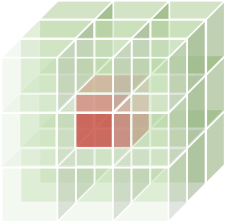
\includegraphics[width=0.4\textwidth]{image/I.png} 
  }
  % \subfigure[图2]
  {
  
\includegraphics[width=0.4\textwidth]{image/J.png}
  }
  
  \label{png1}
\end{figure}


\textbf{Simulation rules:}

\begin{itemize}
  \item Because of the the cause of forest fire is complicated, the fuse may be caused by the careless operation of logging workers, or it may be caused by the trees being struck by lightning. Therefore, we set the initial state of all the cells are 0 or 1, and the initial ignition point generated by the first time slice is arbitrary. All the cells have a certain possibility to become the the first '2' status point.
  \item In the T th time slice, if the states of a unit's southeast corner units are 
  $S_{x+1,y-1,z+1},S_{x+1,y-1,z}$ and $S_{x+1,y-1,z-1}$ 
  , There are $n_1$ burning units in the lower neighborhood, $n_2$ burning units in the middle neighborhood, and $n_3$ burning units in the upper neighborhood (excluding the southeast corner unit), then the combustion tendency K of the $T + 1$ time slice can be expressed as ($f_i$ is the infection probability of the flame in the i-th neighborhood of the cell, $f_3>f_2>f_1$).
  \begin{equation}
    K_{x,y,z}=p\_spread\left [ \frac{n_1f_1}{8}+\frac{n_2f_2}{7}+\frac{n_3f_3}{8}+k_{se}F_{wind}(s_{x+1,y-1,z}+s_{x+1,y-1,z-1}+s_{x+1,y-1,z-1})  \right ] 
  \end{equation}
  The parameter $k_{SE}$ represents the influence weight of southeast wind on fire spread
$p_ {spread}$ is the fire coefficient under considering of different environmental factors, such as temperature, humidity and vegetation type, which represents the comprehensive influence of environmental factors on the spread of forest fire.
  \item When the K value of a cell with state 1 is greater than or equals to B at a time, the cell's state at the next time will turn to 2, and the K value of all units with state 1 will be counted again at each time slice. The interior of the mountain and the air unit are considered to have no combustibles, and the unit without combustibles can not be burned at any time; the burning unit will keep burning all the times after.

\end{itemize}

The above process will continue to repeat until all combustible units are in a burning state, or the spreading trend of the fire is completely blocked by incombustibles. We will observe the spread of the fire rather than the final state, so as to determine the reasonable measures we should take when an extreme fire occurs in Australia, such as adding EOC or increasing the purchase of drones.






\subsection{Model Solving}

Using the altitude data of Victoria, we determined the stadiometry to be about 40km to measure 400km×400km area where the fire was the most serious in Victoria, then we obtained 100 altitude data. We use interpolation method to establish the simplified topographic map of Victoria.

\begin{figure}[H]
  \centering
  {
  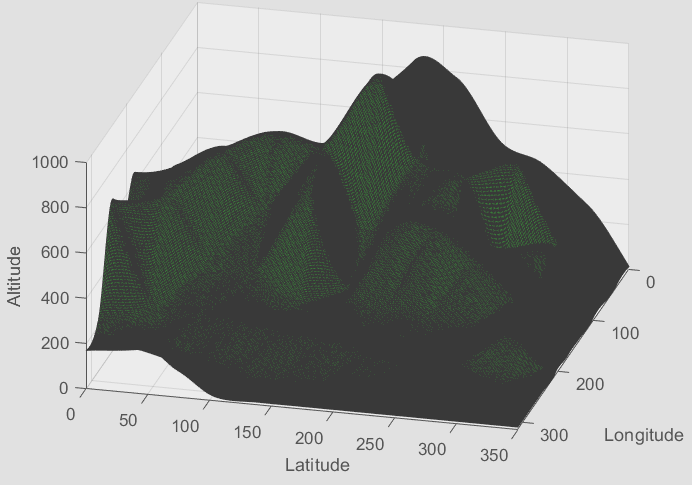
\includegraphics[width=0.4\textwidth]{image/K.png} 
  }
  \label{png1}
\end{figure}

Through matlab simulation, the environmental parameters were adjusted to make the simulation results similar to the spread of forest fires in Victoria from 2019 to 2020. The simulation of the spread of forest fires in the area and the aerial view are as follows:


\begin{figure}[H]
  \centering
  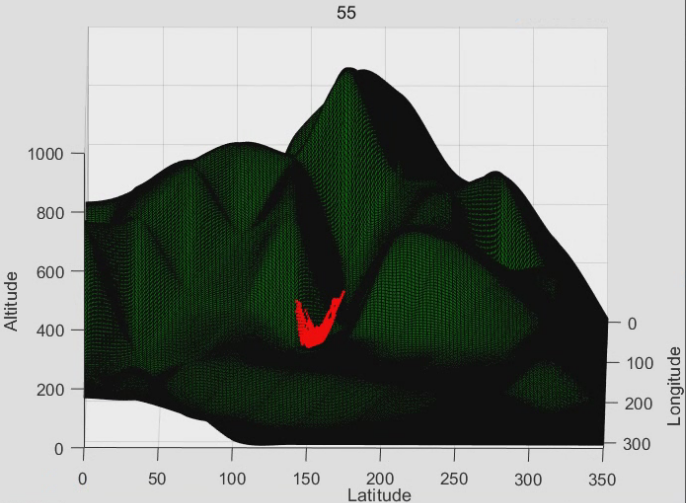
\includegraphics[width=0.2\textwidth]{image/10.png} 
  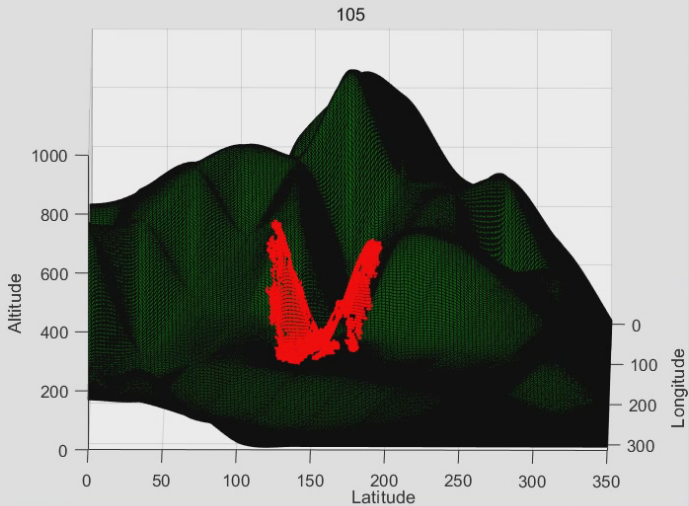
\includegraphics[width=0.2\textwidth]{image/11.png}
  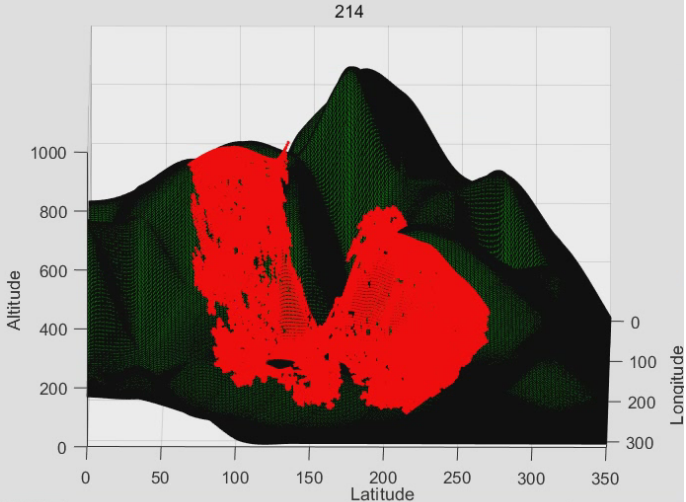
\includegraphics[width=0.2\textwidth]{image/12.png}
  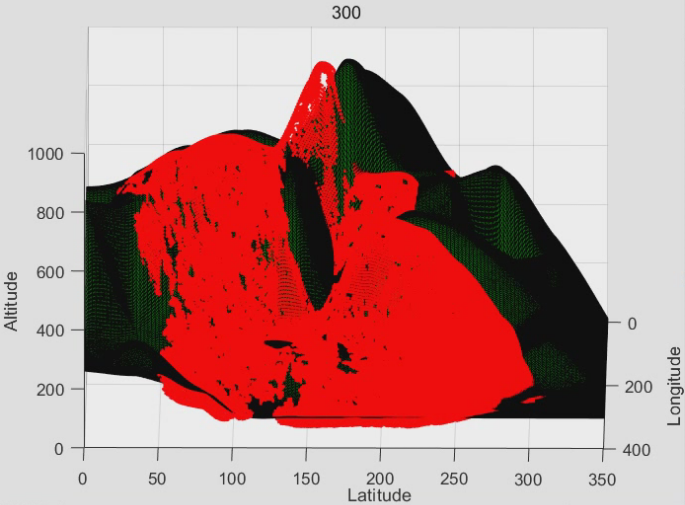
\includegraphics[width=0.2\textwidth]{image/13.png}

  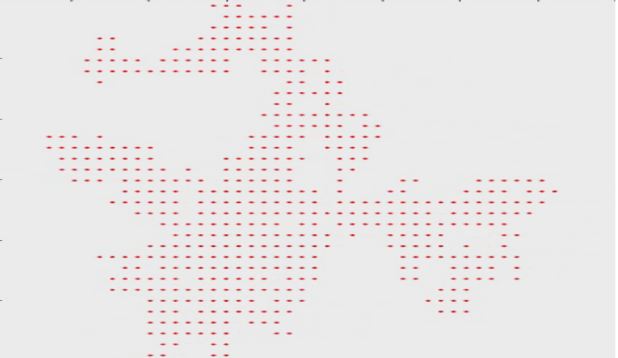
\includegraphics[width=0.2\textwidth]{image/14.png} 
  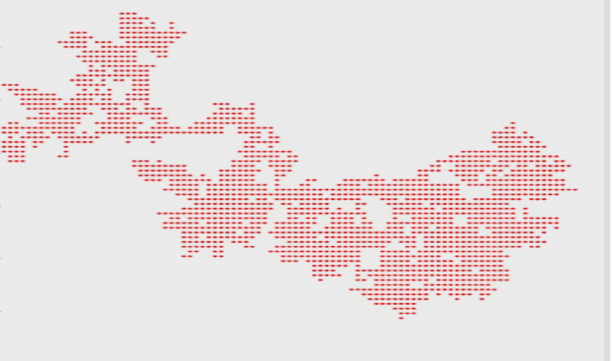
\includegraphics[width=0.2\textwidth]{image/15.png}
  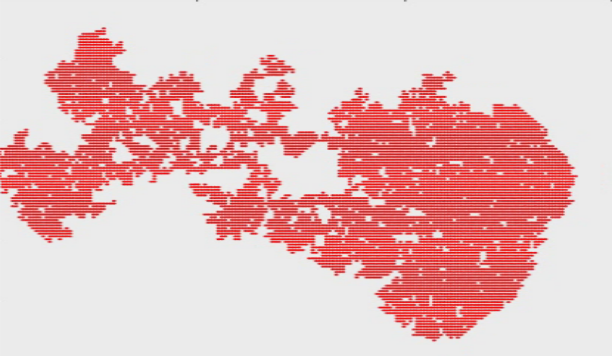
\includegraphics[width=0.2\textwidth]{image/16.png}
  
\includegraphics[width=0.2\textwidth]{image/17.png}
  
  % 
  \label{png1}
\end{figure}

It can be found that according to the topography of the coastal area of Victoria, the early spread of forest fires shows irregular development trend, and the coastal plain area spreads the fastest from northwest to southeast, which is similar to the fire spread law of Victoria in 2019. Therefore, the simulation results of the model can be considered to have reference value. It can be observed that the late fire presents nearly circular coverage, and the higher terrain in the middle were the last to be affected by fire. The spread rate curve of fire behavior with time is as follow :

\begin{figure}[H]
  \centering
  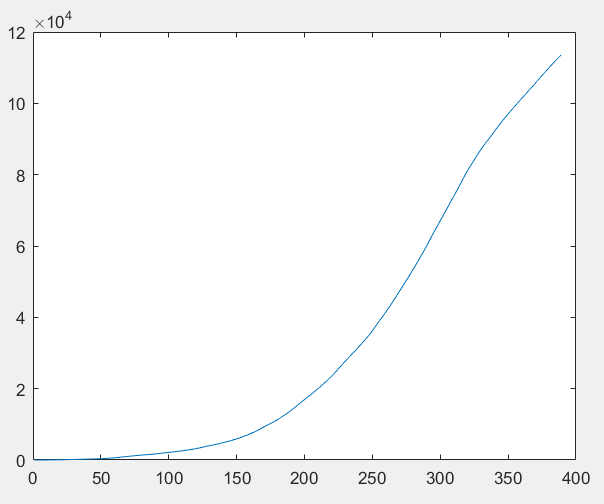
\includegraphics[width=0.4\textwidth]{image/18.png}
  % 
\end{figure}

Therefore, for the purpose of preparing for future rescue missions, we will test the model under the assumption that the fire continues to spread. Due to the difficulty of frequency prediction, according to the simulation results, we replace the frequency index with 0-1 variable to distinguish whether the ignition or not, and then use the program to calculate again. The results show that, taking the 214th time slice as an example, if the fire will spread extremely in the future, it is necessary to add one EOC in the southeast direction and two new repeater drones. However, due to the fact that the fire frequency data is replaced by a 0-1 variable, it is difficult to determine the number of specific SSA drones. If we traverse all flammable points of fire without setting weights according to the frequency, or appropriately delete points with low fire frequency, four SSA drones will be needed.

\subsection{Equipment Cost Increase over the next decade}
Based on the model we built and the predicted fire changes over next decade, we expect to add two repeater drones and four SSA drones. Therefore, the cost of high definition \& thermal imaging cameras, telemetry sensors and repeaters will increase. In addition, in order to achieve the requirements of longer flight time and longer flight distance, we need to increase the cost of power supply systems, navigation systems, and sensors which belong to avionics. The power system needs to increase the cost of electric motors and power batteries. At the same time, due to the expansion of the area to be monitored, we will increase the amount of the emergency operations center, as well as the cost of the ground station control system, ground data terminal and satellite control chain.

\section{Sensitivity Analysis}
An important parameter of our article is the importance weight  $F_{i,j}$ of the flammable point coordinate based on the frequency of fire occurrence. We believe that when the frequency of fire at this point is less than 5 times, set $F_{i,j}$ to 0; when the frequency of fire at this point is between 6 and 100 times, set  $F_{i,j}$ to 1; when the frequency of fire at this point is Between 101 and 300 times, set  $F_{i,j}$ to 1.5; when the frequency of fire at this point is higher than 301 times, set  $F_{i,j}$ to 2. And such a variable setting method is subjective. Therefore, we tried to adjust its weight to 0, 0.5, 1, 1.5, and found that the final EOC position has not changed, so we believe that the model is reliable.

In addition, according to the existing empirical formula, when we calculate obstacles and the distance between the transmitting end and the receiving end of the radio signal, we assume that the path loss index "n" is equal to 3 at the junction of the mountain and the plain. However, there are subjective factors in the setting of the coefficient, so we reset the path loss index to 2.8 and 3.2 respectively.The transmission distance of the repeater corresponding to the 15\% distortion limit does not fluctuate more than 10\%, which means the range is small. Rerun the algorithm After that, the position of the corresponding repeater did not change significantly, so the model is considered reliable.
\section{Strengths and Weaknesses}
\subsection*{9.1 Strengths}
\begin{itemize}
  \item In the determination of EOC and the hovering location of the repeater drone, we fully considered the influence of terrain factors on the communication distance, and drew the fitting curve of the relationship between the communication range radius and the two sides distance,which makes our results more scientific. At the same time, our trone's communication range covers most areas of high fire-prone areas, and can achieve round-the-clock uninterrupted communication in key areas, ensuring the safety of firefighters and the efficiency of information exchange.

  \item We did not choose to predict whether a fire will occur on a specific day, because this requires daily climate data of ten years, and the analysis and processing are more complicated. On the contrary, the monthly average of climate data can better reflect the trend over a period of time, so we choose the monthly climate data of Victoria. In addition, it is still necessary to calculate fire frequency if we predict the fire situation based on daily date. Due to the long-term nature of the next ten years, the monthly forecast can basically achieve the goal. 
\end{itemize}
\subsection*{9.2 Weaknesses}
\begin{itemize}
  \item When predicting the occurrence of fires over the next decade, we cannot predict the specific location of the fire, because we can only obtain climate data of the entire Victoria area, and can only predict the frequency of fires each month in the future. However, it is possible to infer the areas of high risk over the next decade from the fire frequency distribution map in the past ten years.

  \item Due to the lack of parameters in the simulation process of cellular automata, we can only roughly obtain the trend of fire spread in Victoria, but cannot accurately simulate the occurrence of a fire. Although the purpose of using cellular automata is only to predict the general situation of fire spread, it is a pity that we cannot accurately simulate.
\end{itemize}


%--------------------------------
\newpage

\begin{center}
  \textbf{CFA FY 2021 BUDGET REQUEST}
\end{center}

Victoria State Government:

The 2019-2020 fire season in Australia has had a serious impact on our state. In order to better respond to future extreme fire events, we are going to set up a new Rapid Bushfire Response division. The budget supports equipment purchase, scientific and technological research, rescue activities and personnel management to enable the new department to predict and control forest fires. 

\textbf{Equipment}
\begin{itemize}
  \item Purchase wearable devices as personal locator beacons or more complex environmental monitors, and handheld two-way radio communication to give status report and receive orders for forward team.
  \item Purchase of high definition \& thermal imaging cameras and telemetry sensors to monitor and report data from wearable devices on front-line personal.
  \item Purchase of repeaters to extend radio range better communication between front-line personnel and emergency operations centers.
  \item Purchase of Akme Corporation's prototype WileE–15.2X hybrid drone, to carry high definition \& thermal imaging cameras, telemetry sensors and repeaters.A drone is projected to cost approximately \$10,000 (AUD) when equipped with either a radio repeater or video \& telemetry capability.
  \item Maintenance and repair costs of the equipment to ensure that the daily work goes on normally.
\end{itemize}

\textbf{Scientific and Technological}
\begin{itemize}
  \item Studies of Victorian’s topography, climate, plant types and coverage rates, to predict future wildfires.
  \item Studies of drone communications to determine the number and mix of drones which balance capability and safety with economics based on Victoria's topography.
\end{itemize}
\textbf{Rescue Activities}
\begin{itemize}
  \item Purchase of firefighting equipment for forest fire scene rescue.
  \item The cost of shipping support items to the scene of the fire.
  \item The cost of setting up mobile emergency operations center near the site of emergency, including a variety of resources.
  \end{itemize}
\textbf{Personal Management}
\begin{itemize}
  \item The cost of insurance and medical care for forward teams.
  \item Basic costs such as the salaries of deployed personnel and researchers.
  \item Other office and transportation costs. 
\end{itemize}
\begin{flushright}
Victoria’s Country Fire Authority

February 8,2021
\end{flushright}


% 引用文献 %%%%%%%%%%%%%%%%%%%%%%%%%%%%%%%%%%%%%%%%%%%%%%%%%%%%%%%
% \newpage
\bibliography{reference}      % 指定article 代表同目录下的article.bib文件 
\bibliographystyle{ieeetr}  % 定义文献引用的格式
% 附录 %%%%%%%%%%%%%%%%%%%%%%%%%%%%%%%%%%%%%%%%%%%%%%%%%%%%%%%%%
% \begin{appendices}

% \section{First appendix}
% \lipsum[13]
% Here are simulation programmes we used in our model as follow.\\
% \end{appendices}
\end{document}
